\section{Cross-Architecture Experiments}\label{app:arch}

\paragraph{SDXL.} SDXL shares the cross-attention structure of SD v1.4, so
$\hat\kappa$ is directly computable. Table~\ref{tab:sdxl} reports ESD under the
same erasure and evaluation protocol for three concepts. \Cref{fig:umap_sdxl} shows that SDXL's cross-attention activations have qualitatively similar geometry to SD v1.4 (\cref{fig:umap_kappa}): related animal concepts occupy overlapping regions, and \texttt{castle} lies apart from them. Castle's own architectural neighbors are not in this visualization, and its estimated entanglement with them is higher on SDXL ($\hat\kappa_{\text{SDXL}}=0.72$) than on SD v1.4 ($0.27$). The absolute level of entanglement therefore shifts across architectures, but $\hat\kappa$ and observed collateral damage agree within each: on SDXL, NP orders \texttt{cat} $>$ \texttt{castle} $>$ \texttt{dog} exactly as $\hat\kappa_{\text{SDXL}}$ predicts (\cref{tab:sdxl}).

\begin{figure}[h]
\centering
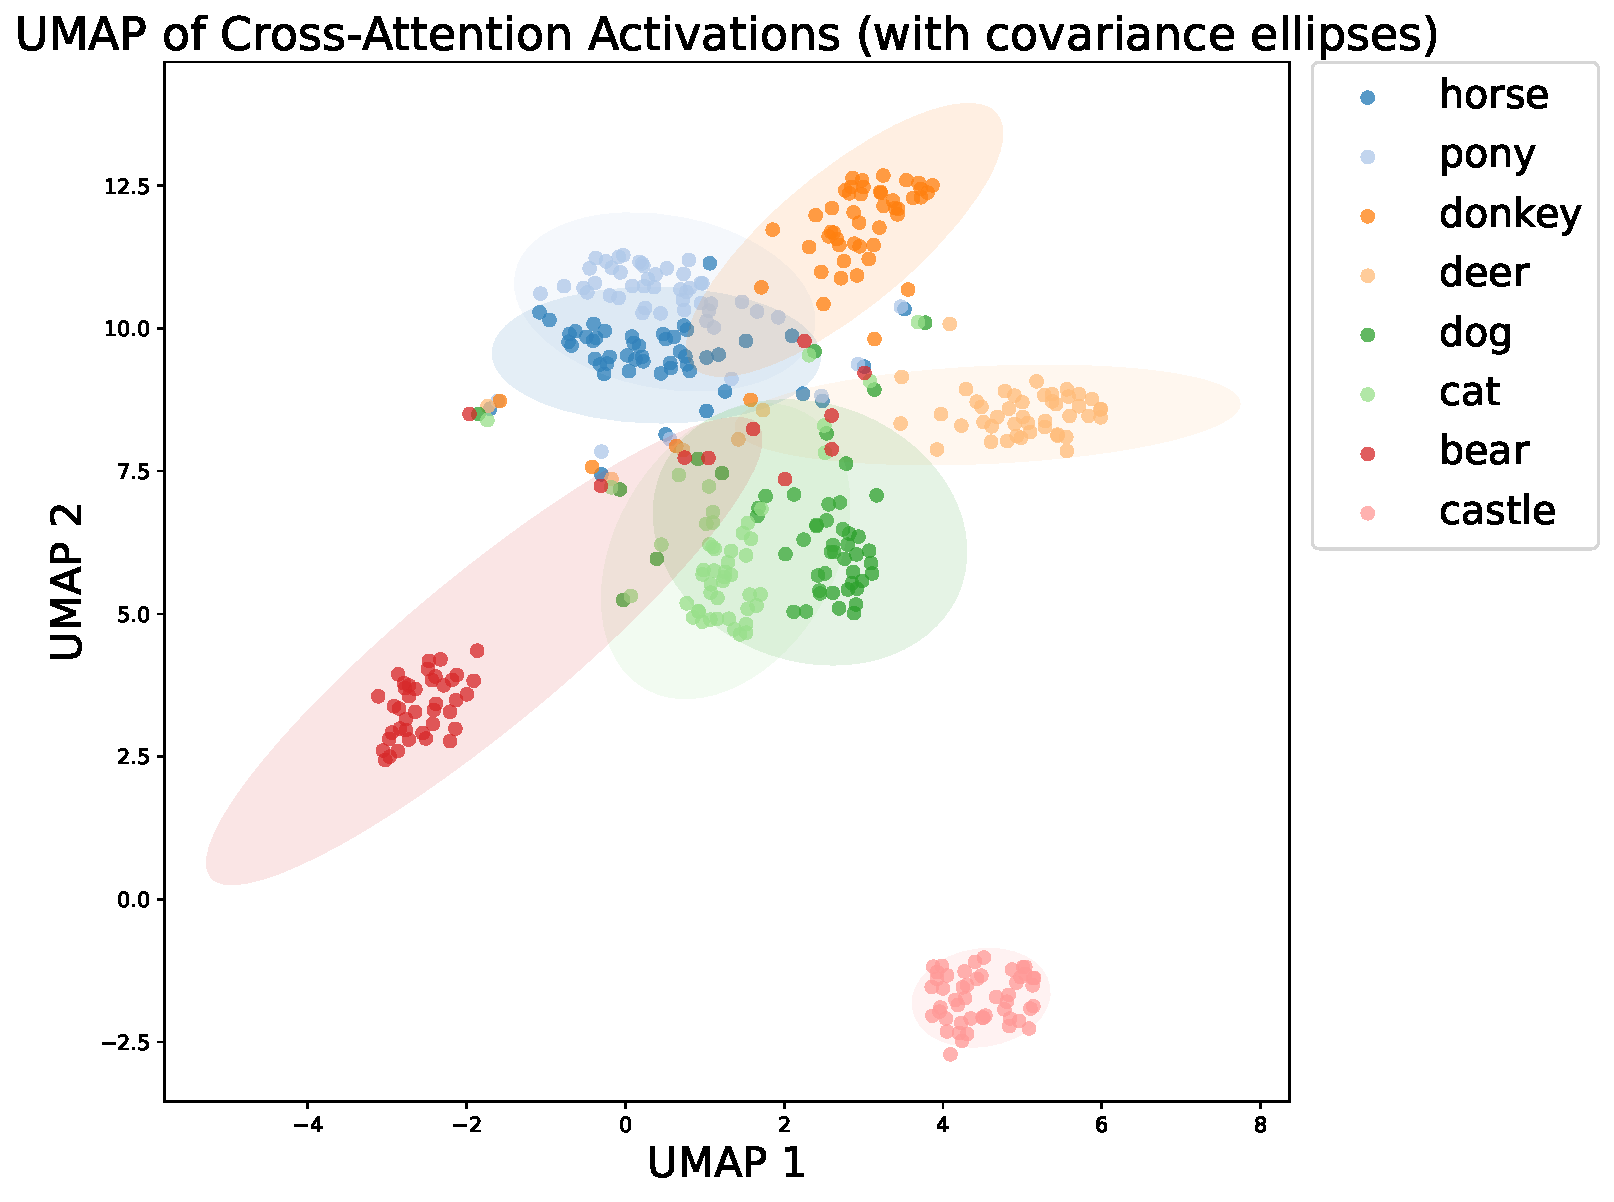
\includegraphics[width=0.7\linewidth]{img/umap_sdxl.pdf}
\caption{UMAP projection of SDXL cross-attention activations for eight
concepts, with covariance ellipses. As in SD v1.4 (\cref{fig:umap_kappa}),
related animal concepts (\texttt{horse}/\texttt{pony}/\texttt{donkey},
\texttt{dog}/\texttt{cat}) overlap, while \texttt{castle} lies apart from the animal clusters. Castle's architectural neighbors are not shown; its entanglement with them is $\hat\kappa_{\text{SDXL}}=0.72$ (\cref{tab:sdxl}).}
\label{fig:umap_sdxl}
\end{figure}

\begin{table}[h]\centering\small
\caption{ESD on SDXL. NP decreases monotonically with $\hat\kappa_{\text{SDXL}}$.}
\label{tab:sdxl}
\begin{tabular}{lcccc}\toprule
Concept & $\hat\kappa_{\text{SDXL}}$ & UA $\uparrow$ & NP $\uparrow$ & DamageGap $\downarrow$\\\midrule
\texttt{cat} & 0.65 & 99 & 90.9 & 9.1\\
\texttt{castle} & 0.72 & 91 & 85.0 & 15.0\\
\texttt{dog} & 0.92 & 77 & 77.1 & 22.9\\\bottomrule
\end{tabular}
\end{table}

\paragraph{FLUX (MMDiT with T5).} FLUX uses joint text-image attention and has
no cross-attention block analogous to \texttt{mid\_block.attentions.0}. A proxy
$\kappa$ estimated from the joint-attention denoiser saturates near $1$ for all
targets (\texttt{dog} $1.00$, \texttt{cat} $0.97$, \texttt{castle} $0.97$) and
also for two unrelated controls (\texttt{airplane}$\to$\texttt{teapot} $0.99$,
bootstrap 95\% CI $[0.94,1.00]$; \texttt{teapot}$\to$\texttt{airplane} $1.00$,
CI $[0.95,1.00]$; centroid distance $0.011$). The proxy therefore does not
resolve concept structure at the layers we can access, and we treat
$\kappa$-scaling on MMDiT as untested. Table~\ref{tab:flux} nonetheless shows
that erasure produces neighbor-selective damage: NP collapses while unrelated
controls are preserved.

\begin{table}[h]\centering\small
\caption{ESD on FLUX (percent).}\label{tab:flux}
\begin{tabular}{lccccc}\toprule
Concept & UA $\uparrow$ & IRR $\downarrow$ & NP $\uparrow$ & CP $\uparrow$ & DamageGap $\downarrow$\\\midrule
Base (\texttt{dog}) & 8.2 & 26.5 & 100.0 & 100.0 & 0.0\\
\texttt{dog} & 78.0 & 8.5 & 35.6 & 96.9 & 61.3\\
\texttt{cat} & 83.0 & 9.5& 37.8 & 95.3 & 57.6\\
\texttt{castle} & 85.0 &20.0 & 40.5 & 98.9 & 58.3\\\bottomrule
\end{tabular}
\end{table}

\paragraph{Comparison across backbones.} For ESD on \texttt{dog}, erasure is
nearly matched across backbones (UA $75$, $77$, and $78$ on SD v1.4, SDXL, and
FLUX), while NP is $93.5$, $77.1$, and $35.6$. The robustness-retention
trade-off therefore persists on newer backbones rather than being specific to
SD v1.4. Absolute NP is not strictly comparable across architectures because
their image distributions differ.
